\documentclass[10pt,a4paper]{article}
\usepackage[T1]{fontenc}
\usepackage{amssymb}
\usepackage[left=15mm,right=15mm,top=20mm,bottom=27mm]{geometry}
\usepackage{graphicx}
\usepackage{isabelle}
\usepackage{isabellesym}
\usepackage[only,bigsqcap]{stmaryrd}
\usepackage{pdfsetup}

\urlstyle{tt}
\isabellestyle{tt}

\renewcommand{\isacharunderscore}{\_}
\renewcommand{\isachardoublequoteopen}{``}
\renewcommand{\isachardoublequoteclose}{''}

\begin{document}

\title{Soundness of the Q0 proof system for higher-order logic}
\author{Anders Schlichtkrull}
\date{}

\maketitle

\begin{abstract}
\noindent
This entry formalizes the Q0 proof system for higher-order logic (also known as simple type theory) from
the book ``An Introduction to Mathematical Logic and Type Theory: To Truth Through Proof'' 
by Peter B. Andrews \cite{andrews2013introduction} together with the system's soundness.
Most of the used theorems and lemmas are also from his book.
The soundness proof is with respect to general models and as a consequence also holds for standard models.
Higher-order logic is given a semantics by porting to Isabelle/HOL the
specification of set theory from the CakeML project \cite{DBLP:conf/itp/KumarAMO14,DBLP:journals/jar/KumarAMO16}.
The independently developed AFP entry ``Metatheory of Q0'' by Javier D{\'i}az \cite{Q0_Metatheory-AFP} also formalizes Q0 in Isabelle/HOL. 
I highly recommend the reader to also take a look at his formalization!
\end{abstract}

\tableofcontents

\newpage

% sane default for proof documents
\parindent 0pt
\parskip 0.5ex

\section{Introduction}
This entry formalizes the Q0 proof system for higher-order logic (also called simple type theory)
and its soundness.
Both the system and most of the proven lemmas and
theorems are from Peter B. Andrews' book \cite{andrews2013introduction}.
In the book's chapter on type theory, Andrews explains that type theory was invented by
Russell \cite{russell1908mathematical} and that Whitehead and Russell \cite{whiteheadrussel} showed that fundamental
parts of mathematics could be formalized in type theory.
As influences on the type theory presented in Andrews' chapter he mentions Church \cite{church1940formulation}, Henkin \cite{henkin1950completeness,henkin1963b} and earlier works by himself \cite{andrews1963reduction,andrews1972general}.
The present Isabelle formalization of higher-order logic is given a semantics by using a port to Isabelle/HOL of 
CakeML's specification of set theory \cite{DBLP:journals/jar/KumarAMO16}.
The specification is formalized as a locale that fixes a type of set theoretic sets
and a number of functions (powerset, union, separation) and the set membership predicate.
The soundness proof is with respect to general models and as a consequence it also holds for standard models.
Variables are implemented simply using named variables rather than e.g.\ De Bruijn indices or nominal techniques.
It is well-known that named variables require the definition of substitution to rename variables, but since
substitution is derived in Q0 rather than built into the proof system this complication is essentially
circumvented in the present formalization. 
As a curiosity the present AFP entry also proves that the set theory specification is fulfilled
by the sets axiomatized in Isabelle/HOLZF \cite{DBLP:conf/ictac/Obua06} and also by the sets axiomatized by the
AFP entry on Zermelo Fraenkel Set Theory in Higher-Order Logic \cite{ZFC_in_HOL-AFP}.
The theory files of the present entry appeared in the IsaFoL effort \cite{Q0IsaFoL}.

In the literature we find other formalizations of the metatheory of higher-order logics and type theories.
Independently from my work here, Javier Díaz also formalizes Q0 in Isabelle/HOL.
His work is available in the AFP entry ``Metatheory of Q0'' \cite{Q0_Metatheory-AFP}. 
I highly recommend the reader to take a look also at his very thorough formalization!
Arthan specifies HOL \cite{arthan1993,arthan1991sem,arthan1991ded} in ProofPower but does not prove soundness.
John Harrison formalizes the soundness of the proof system of HOL Light \cite{DBLP:conf/cade/Harrison06} in HOL Light
and Kumar et al.\ \cite{DBLP:conf/itp/KumarAMO14,DBLP:journals/jar/KumarAMO16,DBLP:conf/itp/AbrahamssonMKS22,DBLP:conf/itp/AbrahamssonM23} formalize 
it in HOL4 as part of the CakeML project including also definitions and a verified implementation.
Ro{\ss}kopf and Nipkow \cite{DBLP:conf/cade/NipkowR21,Metalogic_ProofChecker-AFP,DBLP:journals/jar/RosskopfN23}
formalize a proof system for terms in Isabelle's metalogic together with an implementation of a 
proof checker and prove that the proof checker indeed implements this proof system.
There are also a number of works using Coq to formalize metatheory of the calculus of constructions and
the calculus of inductive constructions \cite{DBLP:conf/types/Barras96,barras:inria-00073667,coqincoqmanuscript,coqincoqcontribs,DBLP:journals/pacmpl/SozeauBFTW20}.
Worth mentioning is also the formalization in Coq of second-order logic which also formalizes general models \cite{DBLP:conf/cpp/KochK22}.

There are plenty of opportunities to go further with the present formalization.
The present formalization proves soundness of Q0 theorems (i.e. $\vdash A$ implies $\models A$), but not 
soundness of Q0 derivability (i.e. $M \models G$ and $G \vdash A$ implies $M \models A$).
Other interesting lemmas and theorems from Andrews' book could also be proved such as e.g.\ derived inference rules and completeness.

\begin{figure}
\begin{center}
  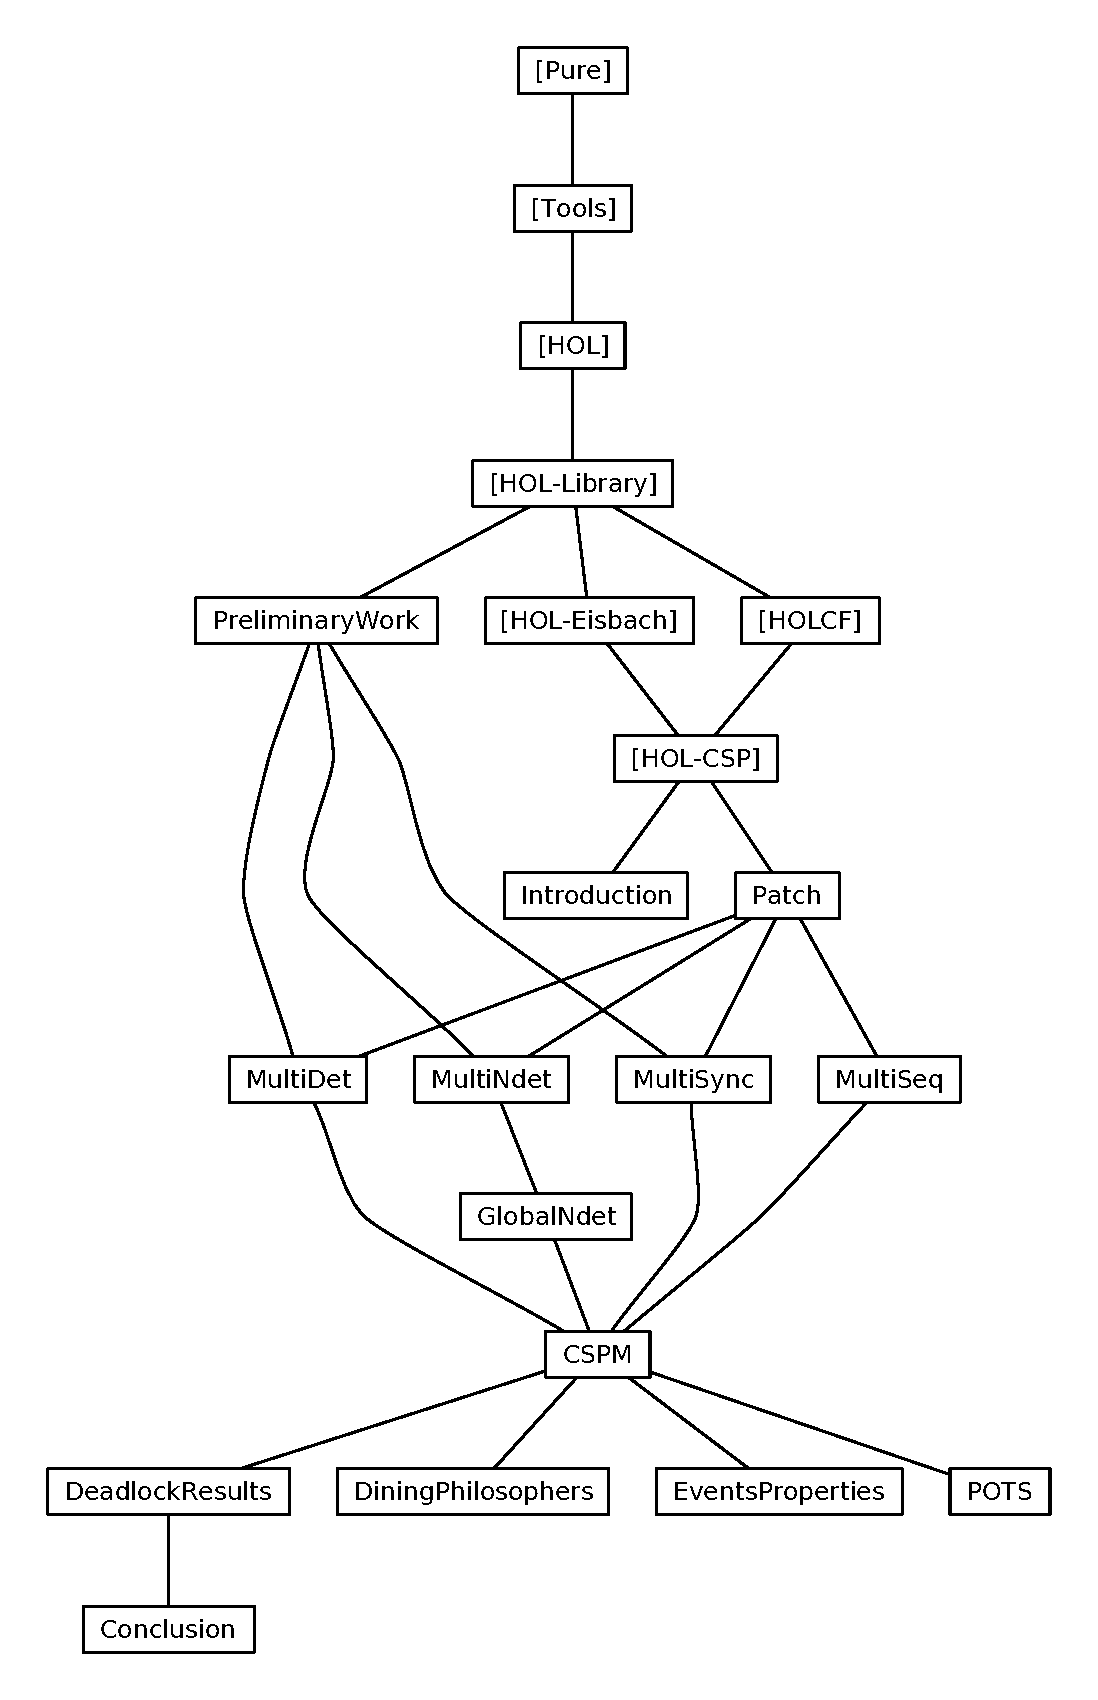
\includegraphics[width=0.4\textwidth,keepaspectratio]{session_graph}
\end{center}
\caption{Theory dependency graph}
\label{fig:thys}
\end{figure}

\newpage

% generated text of all theories
\input{session}

% optional bibliography
\bibliographystyle{alpha}
\bibliography{root}

\end{document}
